%27/09 - Luis del Peso
\chapter{Modelos estadísticos en el análisis de secuencias}
%Hay dos modelos estadísticos fundamentales para el análisis de secuencias: el modelo multinominal y la cadena de Markov. 
En biología existen tres tipos fundamentales de secuencias: ADN, ARN y aminoácidos. Estas secuencias representan el núcleo del dogma central de la biología molecular, ya que almacenan toda la información genética necesaria para perpetuar la vida. No obstante, el análisis de estas secuencias presenta una gran complejidad debido a su estructura y funcionalidad. Aunque son polímeros lineales formados por un número limitado de subunidades o monómeros, la disposición específica de estas subunidades a lo largo de la molécula es clave para su función. Debido a su estructura química, estas secuencias pueden representarse como cadenas de símbolos, lo que permite su estudio utilizando herramientas matemáticas y computacionales.

\section{Modelo multinomial}
Desde un enfoque matemático, las secuencias biológicas pueden verse como una concatenación de símbolos provenientes de un alfabeto definido: en el caso del ADN, el alfabeto es ATCG; en el ARN, AUCG; y en las proteínas, está compuesto por 20 aminoácidos. Formalmente, una cadena es una secuencia finita de símbolos de un alfabeto $\Sigma$. Así, $\Sigma^3$ representa todos los codones posibles dentro del código genético.

\textit{Ejemplo práctico:}
Consideremos un ejercicio de modelización estadística aplicado al ADN. En un experimento ChIP-seq (una técnica de secuenciación masiva que permite identificar sitios de unión de proteínas al ADN), se descubrieron 500 sitios de unión para un factor de transcripción. Dado que el genoma humano contiene entre 20,000 y 26,000 genes, estos 500 sitios parecen pocos. Sin embargo, la cuestión central es si esta cantidad es coherente con lo que se esperaría bajo un modelo estadístico.
Los factores de transcripción se unen a subsecuencias específicas de ADN llamadas "motivos de respuesta". En este caso, el motivo de unión es RCGTG, donde R representa A o G. Aunque las moléculas biológicas interaccionan con cierta flexibilidad, este motivo es bastante restringido, ya que solo una posición es flexible. El genoma humano tiene alrededor de $3 \times 10^9$ bases, por lo que podemos calcular la cantidad esperada de sitios de unión basándonos en la probabilidad de que este motivo ocurra aleatoriamente.
Asumiendo que los nucleótidos son independientes entre sí y tienen la misma probabilidad de aparecer, la probabilidad de que aparezca la secuencia CGTG es $0,25^4$. Para la posición R, que puede ser A o G, la probabilidad es $0,5$. Por tanto, la probabilidad total de encontrar el motivo RCGTG es $0,25^4 \times 0,5 = \frac{1}{512}$, es decir, se esperaría encontrar esta secuencia una vez cada 512 posiciones. Con un genoma de $3 \times 10^9$ bases, se esperaría aproximadamente $\frac{3 \times 10^9}{512} \approx 6 \times 10^6$ sitios. Sin embargo, en el experimento solo se hallaron 500 sitios, lo que sugiere que el modelo experimental no refleja completamente la realidad biológica y es necesario recurrir a otros modelos, aunque sean simplificados.
La secuencia por sí sola no es suficiente para que el factor de transcripción se una. Otros factores, como la accesibilidad de la cromatina, también juegan un papel crucial. No obstante, el modelo multinomial proporciona una referencia útil para evaluar los datos experimentales en un contexto aleatorio.
En este modelo multinomial, se asume que los nucleótidos en cada posición son independientes y tienen la misma probabilidad de aparecer (hipótesis nula), lo que simplifica los cálculos:

 $$ \prod_{i=1}^{n} p(s_i) $$

Si bien este enfoque es sencillo, tiene limitaciones significativas, como la suposición de independencia entre nucleótidos. Sabemos que esto no es siempre cierto, por ejemplo, los dinucleótidos CG suelen ser menos frecuentes salvo en las "islas CpG", donde existe una gran concentración.

\subsection{Frecuencia de dinucleótidos}
Los dinucleótidos, que representan todas las combinaciones posibles de dos nucleótidos ($\Sigma^2$), deberían tener una frecuencia esperada de $\frac{1}{16}$ en el genoma humano. Al analizar las frecuencias observadas en el cromosoma 21, se encuentra que A y T aparecen con una frecuencia del 29.5\%, mientras que G y C con un 20.5\% (Figura \ref{fig:dinucleotidos}). Al recalcular las frecuencias de los dinucleótidos, se observa que, en general, la frecuencia observada coincide con la esperada, excepto para el dinucleótido CG, cuya frecuencia observada es tres veces menor a la esperada. Esto sugiere que los nucleótidos no son completamente independientes, y el modelo multinomial no es suficiente para describir esta dependencia.

\begin{figure}[htbp]
\centering
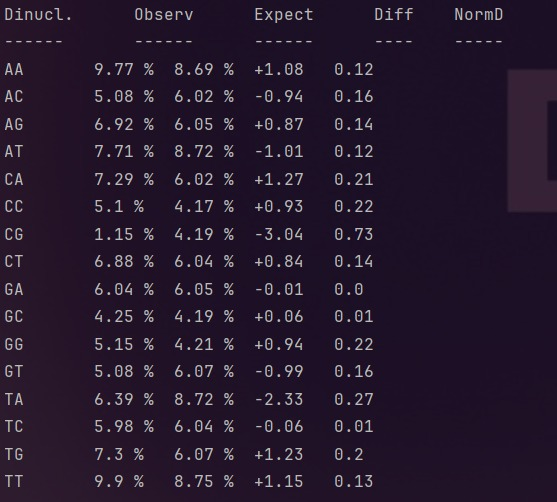
\includegraphics[width = 0.55\textwidth]{figs/freqs-dinucleotidos.jpg}
\caption{Cálculo de las frecuencias de los 16 dinucleótidos en el cromosoma 21 del ser humano. Los valores esperados y observados suelen coincidir en $\pm$ 1\% a excepción del dinucleótido CG. }
\label{fig:dinucleotidos}
\end{figure}
 
\section{Cadena de Markov}
Para modelar adecuadamente fenómenos como las islas CpG, es necesario utilizar un enfoque diferente: las cadenas de Markov. En estos modelos, cada posición en la secuencia de ADN se considera un "estado" que corresponde a uno de los cuatro nucleótidos, y la probabilidad de que un nucleótido aparezca en una posición depende del nucleótido anterior. Este tipo de dependencia se representa mediante una matriz de transición que contiene las probabilidades condicionales de pasar de un nucleótido a otro (Figura \ref{fig:markov}). Matemáticamente, un modelo de Markov de primer orden puede expresarse de la siguiente manera:

 $$ p(s_1) * \prod_{i=2}^{n} p(s_i | s_{i-1}) $$
 
\begin{figure}[htbp]
\centering
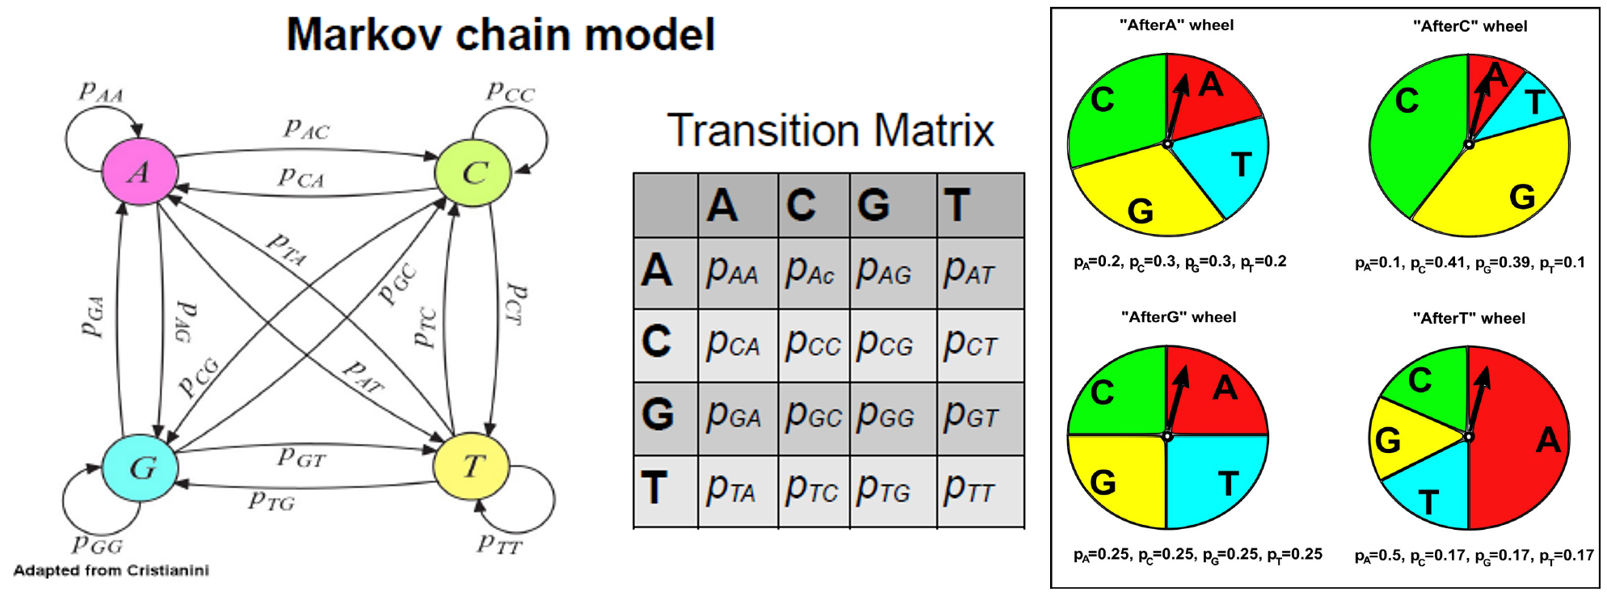
\includegraphics[width = 0.7\textwidth]{figs/markov.png}
\caption{Representaciones gráficas de la cadena de Markov. En la matriz de transición, las filas corresponden a los nucleótidos de la posición anterior y las columnas los nucleótidos que les siguen. }
\label{fig:markov}
\end{figure}
 
Por ejemplo, para calcular la probabilidad de encontrar la secuencia RCGTG utilizando este modelo, se deben considerar las probabilidades condicionales para cada posible combinación de nucleótidos. La probabilidad se calcula dividiendo la secuencia en dos casos, que luego se suman:
\begin{align*}
0,25 \times 0,3 \times 0,39 \times 0,25 \times 0,17 (ACGTG) \\
+ 0,25 \times 0,25 \times 0,39 \times 0,25 \times 0,17 (GCGTG) \\
= 0,001243 + 0,001036 \\
= 0,002279 
\end{align*}
 
\textbf{Problema práctico:}
Un desafío interesante sería escribir un programa que identifique islas CpG en un fragmento del genoma humano. Los dinucleótidos CG tienden a perderse debido a la metilación de la citosina, que, al desaminarse, se convierte en timina en lugar de regresar a citosina. Sin embargo, en regiones del genoma que no se metilan, como las regiones transcripcionalmente activas, las secuencias CG permanecen intactas, formando las llamadas islas CpG. El objetivo del programa sería localizar el inicio y el final de una de estas islas en una secuencia genómica.
\begin{figure}[htbp]
\centering
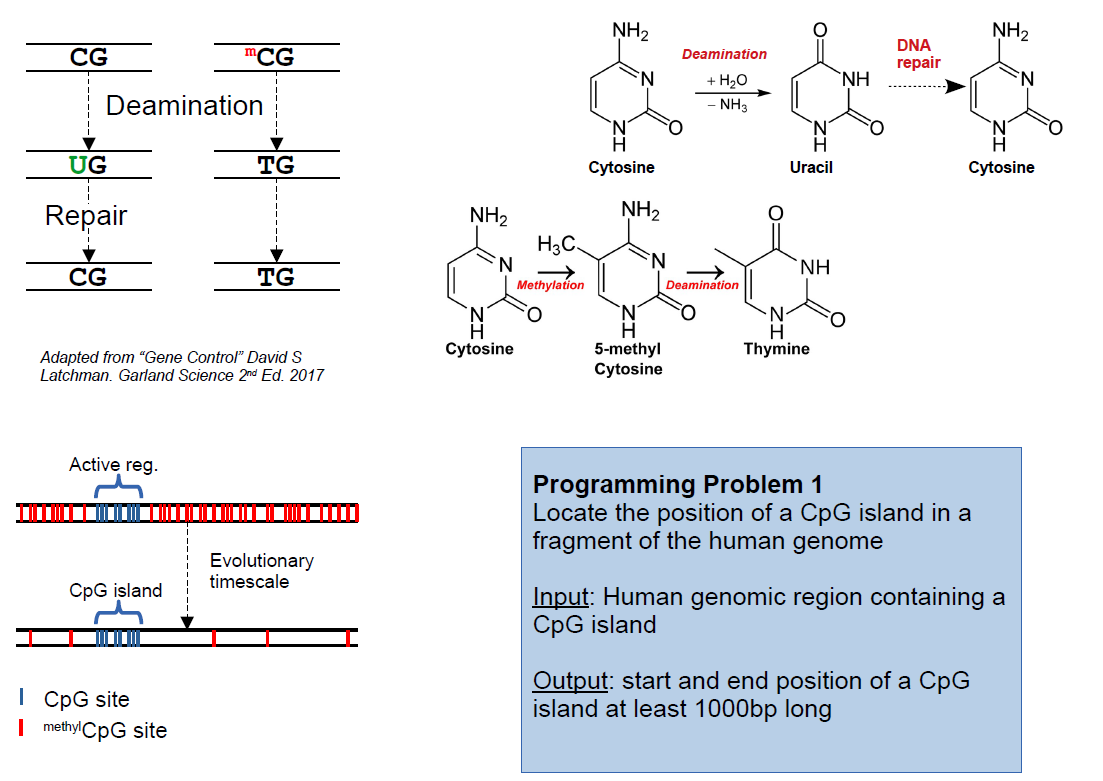
\includegraphics[width = 0.7\textwidth]{figs/cpg-islands.png}
\caption{Explicación biológica gráfica de las islas CpG. }
\end{figure}
 